\renewcommand*{\arraystretch}{1.1}

\noindent\begin{tabularx}{17cm}{|>{\small \sf}c|X|}
	\hline
	query    & Interactive / update / 7 \\ \hline
%
	title       & Add Comment \\ \hline
%
    pattern     & \hfill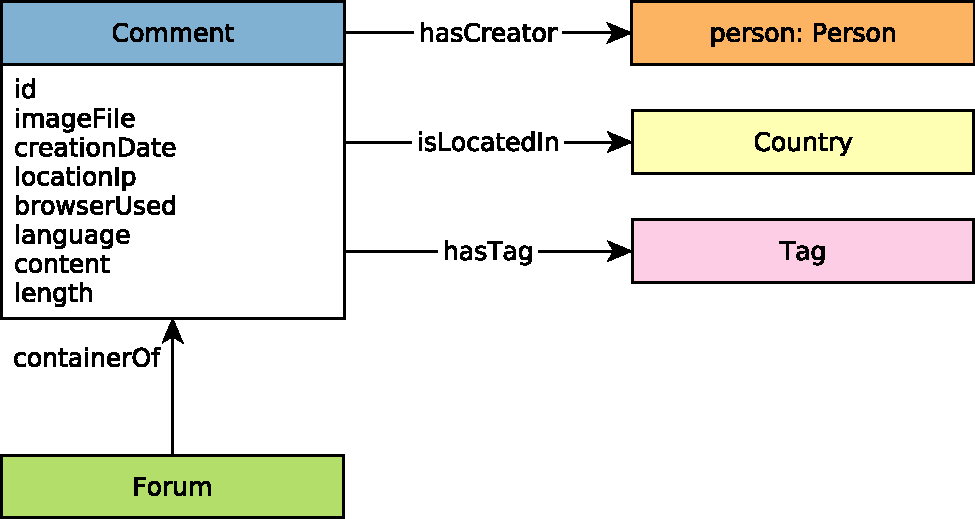
\includegraphics[scale=\patternscale,margin=0cm .2cm]{patterns/interactive-update-07}\hfill\vadjust{} \\ \hline
%
	desc. & Add a Comment replying to a Post/Comment to the social network.
 \\ \hline
%
	
%
	params.  &
	\vspace{1.1ex}{\begin{tabularx}{14.2cm}{|c|M|m{2cm}|Y|} \hline
	\cellcolor{parameter} \color{white} $\mathsf{1}$ & \varname{Comment.id} & \cellcolor{gray!20} \vartype{ID} &  \\ \hline
	\cellcolor{parameter} \color{white} $\mathsf{2}$ & \varname{Comment.creationDate} & \cellcolor{gray!20} \vartype{DateTime} &  \\ \hline
	\cellcolor{parameter} \color{white} $\mathsf{3}$ & \varname{Comment.locationIp} & \cellcolor{gray!20} \vartype{String} &  \\ \hline
	\cellcolor{parameter} \color{white} $\mathsf{4}$ & \varname{Comment.browserUsed} & \cellcolor{gray!20} \vartype{String} &  \\ \hline
	\cellcolor{parameter} \color{white} $\mathsf{5}$ & \varname{Comment.content} & \cellcolor{gray!20} \vartype{Text} &  \\ \hline
	\cellcolor{parameter} \color{white} $\mathsf{6}$ & \varname{Comment.length} & \cellcolor{gray!20} \vartype{32-bit Integer} &  \\ \hline
	\cellcolor{parameter} \color{white} $\mathsf{7}$ & \varname{Comment-hasCreator->Person.id} & \cellcolor{gray!20} \vartype{ID} &  \\ \hline
	\cellcolor{parameter} \color{white} $\mathsf{8}$ & \varname{Comment-isLocatedIn->Country.id} & \cellcolor{gray!20} \vartype{ID} &  \\ \hline
	\cellcolor{parameter} \color{white} $\mathsf{9}$ & \varname{Comment-replyOf->Post.id} & \cellcolor{gray!20} \vartype{ID} & $-1$ if the comment is a reply of a comment \\ \hline
	\cellcolor{parameter} \color{white} $\mathsf{10}$ & \varname{Comment-replyOf->Comment.id} & \cellcolor{gray!20} \vartype{ID} & $-1$ if the comment is a reply of a post \\ \hline
	\cellcolor{parameter} \color{white} $\mathsf{11}$ & \varname{\{Comment-hasTag->Tag.id\}} & \cellcolor{gray!20} \vartype{\{ID\}} &  \\ \hline
	\end{tabularx}}\vspace{1.1ex} \\ \hline
%
	
%
	%
	%
	%
    %
\end{tabularx}
\vspace{2ex}